%------------------------------- CHAPTER NAME --------------------------------
\chapter{Specific Range and Cruise Grid}
In this chapter an anlysis of the specific range is performed with the aim of obtain useful information about cruise performance. 

In particular, starting from generalized performance evaluation and interfacing them with the fuel consumption, the final objective will be to define the specific range as function of Mach number, obtaining the so called \emph{cruise grid chart} which is a very important tool for pilots because it allows to choose the correct speed, during cruising phase, in order to follow some mission objectives like minimum fuel consumption or a fast cruise.

%-------------------------- THEORETICAL BACKGROUND ---------------------------
\section{Theoretical background}
The first step that has to be done in order to obtain the \emph{cruise grid chart} is to define generalized performance in terms of thrust and drag. The \emph{generalized} attribute given to these quantities stands for the fact that they are independents from altitude and this result is reached through the parameter $\delta$ which represents a ratio between the total pressure at compressor inlet and  the standard pressure at sea level. 

\bigskip
\noindent
Regarding the thrust, the generalized version can be obtained by dividing it by $\delta$ as shown below.
\begin{equation}
\frac{T}{\delta}=\frac{T_{f}}{\delta}-M\cdot a_{0}\cdot \frac{\sqrt{\theta \cdot m_{a}}}{\delta}
\label{eqn:Equation1}
\end{equation}

\begin{figure}[!ht]
\centering
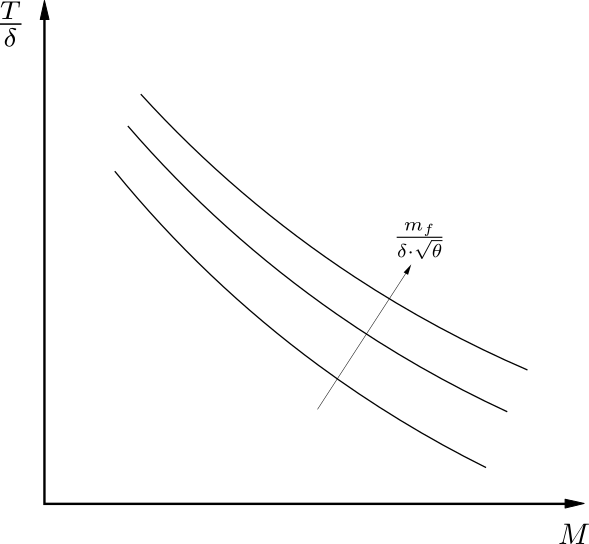
\includegraphics[keepaspectratio, width=0.50\textwidth]{TDelta}
\caption{Qualitative trend of  the generalized thrust v.s. Mach number parameterized in generalized fuel flow rate}
\label{fig:Figure1}
\end{figure}

\noindent
where

\begin{itemize}
\item $T$, is the net thust
\item $T_{f}$, is the gross thrust
\item $M$, is the mach number
\item $a_{0}$, is the sound speed at sea level
\item $\dfrac{\sqrt{\theta \cdot m_{a}}}{\delta}$, is the genralized air flow rate which is function of the generalized fuel flow rate given by $\dfrac{m_{f}}{\delta \cdot \sqrt{\theta}}$
\end{itemize}

\noindent
so that the genralized thrust results as a function of Mach number and generalized fuel flow rate.

\begin{equation}
\frac{T}{\delta}=\frac{T_{f}}{\delta}\cdot f\left(\frac{m_{f}}{\delta \cdot \sqrt{\theta}}\right)
\label{eqn:Equation2}
\end{equation}

\bigskip
\noindent
As shown in figure~\ref{fig:Figure1} the generalized thrust decreases with Mach number, at given fuel flow rate, and grows with the latter, at given Mach number. This because if the Mach number grows at fixed fuel flow rate, the air flow rate grows reducing the thrust; otherwise, if fuel flow rate grows at fixed Mach number, air flow rate is lower giving more thrust.

With this function it's possible to correlate generalized thrust to hourly fuel consumption which is a main keypoint in building the cruise grid chart of an endurance based aircraft such as UAV. 

Since transport aircrafts rely more on range performance, it's necessary to obtain the same relationship between generalized thurst and fuel consumption referred to the generalized specific range indicated with $\delta\bar s $. 

\bigskip
\noindent
Dividing the generalized fuel flow rate, which is dimesionally equal to $\frac{\si{\kilogram}}{\second}$, by a velocity, the result has a dimension of $\frac{\meter}{\si{\kilogram}}$ that represents the reciprocal of the specific range. In this way it's possible to state the following relation.

\begin{equation}
\frac{m_{f}}{\delta \cdot \sqrt{\theta}}=\frac{M\cdot a_{0}}{\delta\bar s}
\label{eqn:Equation3}
\end{equation}

\begin{figure}[!ht]
\centering
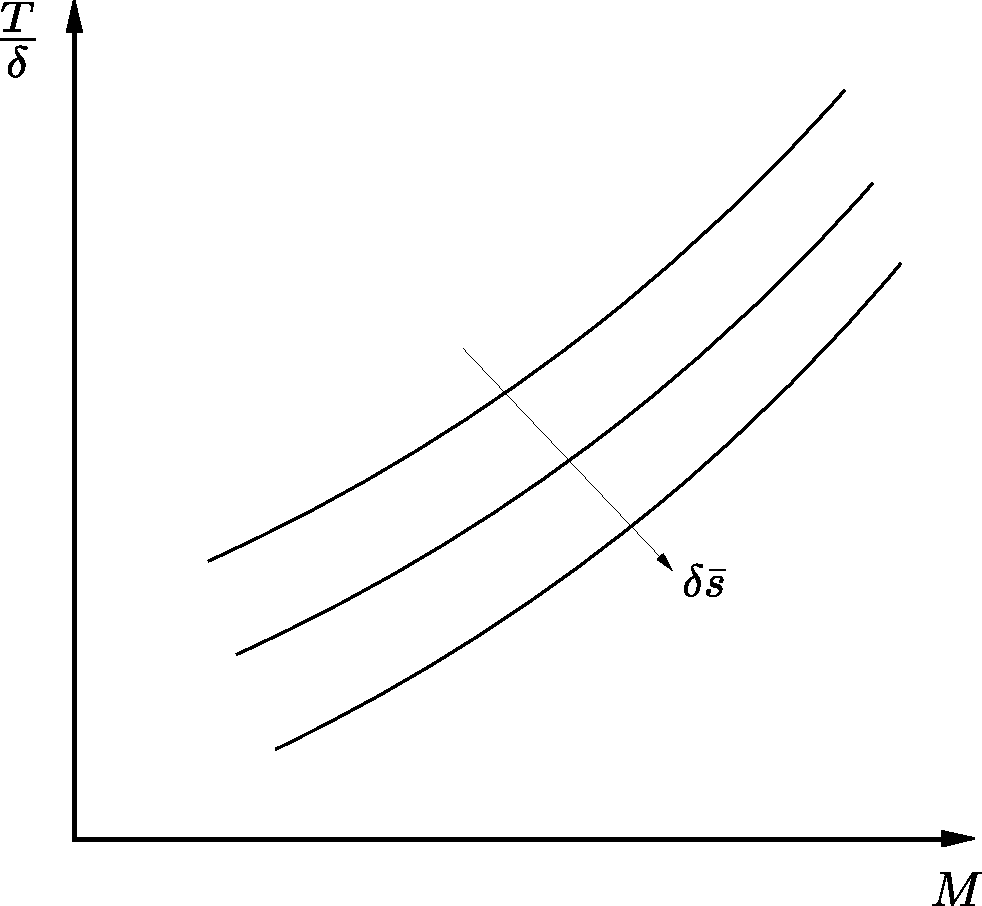
\includegraphics[keepaspectratio, width=0.50\textwidth]{TDelta_SpecificRange}
\caption{Qualitative trend of the generalized thrust v.s. Mach number parameterized in generalized specific range}
\label{fig:Figure2}
\end{figure}

\bigskip
\noindent
As expectd from the relation (\ref{eqn:Equation3}) the thrust has a trend which is the inverse of the previous parameterization. In fact now, for a given Mach number, if the pilot wants to go farther he has to decrease the thrust in order to reduce the fuel consumption; otherwise, at a given distance to reach, the pilot has to increase the thrust in order to make the Mach number grows.

\bigskip
\noindent
Since the thrust has always to be compared with the drag in order to evaluate if the aircraft can fly in a specific cruise condition without loosing speed and altitude, it's necessary to obtain a generalized drag trend as well. 

This ai very similar to the drag trend, as can be seen from figure~\ref{fig:Figure3}, and it depends from aircraft weight as well; but, since these have to be generalized quantities, the weight is a generalized weight too.

\begin{figure}[b]
\centering
\includegraphics[keepaspectratio, width=0.50\textwidth]{DragDelta_SpecificRange}
\caption{Qualitative trend of the generalized drag v.s. Mach number parameterized in generalized weight}
\label{fig:Figure3}
\end{figure}

\bigskip
\noindent
By the overlap of figure~\ref{fig:Figure2} and figure~\ref{fig:Figure3} charts, it's easy to note that the best Mach number, for a given generalized weight, is located at the intersection of the two curves as reported in figure~\ref{fig:Figure4}. In fact, in order to obtain a bigger specific range at fixed weight, the generalized drag would be higher than the generalized thrust; otherwise, if the pilot wants to fly faster at given weight, he has to increase thrust so that the specific range will decrease due to the increasing fuel consumption.

Since during the cruise phase the aircraft weight decreases continuously, the pilot has to gain altitude in order to leave the generalized weight unchanged; this explains why during cruise the aircraft continues to climb. 

\begin{figure}[t]
\centering
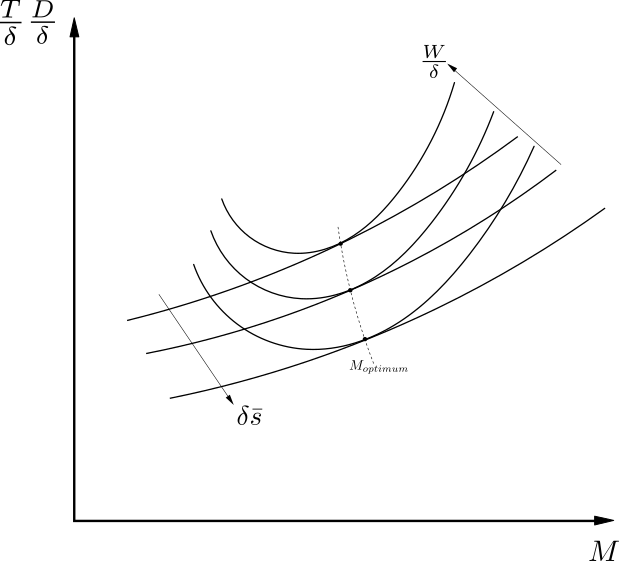
\includegraphics[keepaspectratio, width=0.50\textwidth]{TDeltaDragDelta}
\caption{Comparison between generalized drag and generalized thrust as functions of Mach number}
\label{fig:Figure4}
\end{figure}

\bigskip
\noindent
The specific range can also be connected to Breguet formulas (\ref{eqn:BreguetEquation}) as it can be obtained by dividng the autonomy factor, $A.F.$, by the aircraft weight; in particular the autonomy factor, groups three main aircraft efficiency and can be written as follow.

\begin{subequations}\label{eqn:AutonomyFactor}
\begin{equation}\label{eqn:AutonomyFactorProp}
A.F.=
      \begin{array}{l@{\rule{5em}{0pt}}l} 
      \dfrac{\eta_{p}}{SFC}\cdot\left(\dfrac{L}{D}\right)
          & \text{if} \;\, \text{propeller engine driven}
      \end{array}
\end{equation}
\begin{equation}\label{eqn:AutonomyFactorJet}
A.F.=
      \begin{array}{l@{\rule{7em}{0pt}}l} 
      \dfrac{V}{SFCJ}\cdot\left(\dfrac{L}{D}\right)
          & \text{if} \;\, \text{jet engine driven}
      \end{array}
\end{equation}
\end{subequations}

\noindent
where

\begin{itemize}
\item $\eta_{p}$, is propeller efficiency
\item $SFC$, is related to propulsive efficiency
\item $\left(\frac{L}{D}\right)$, is the aerodynamic efficiency
\end{itemize}

\noindent 
At given generalized weight and generalized specific range, the optimum Mach is known as explained before and so the autonomy factor can be calculated by multiply $\frac{W}{\delta}$ and $\delta\bar s$. Repeating this operation for different generalized weight conditions, allows to define the autonomy factor trend as function of the generalized weight in which each point of the chart is related to an optimum Mach number for the specific range.

\begin{figure}[t]
\centering
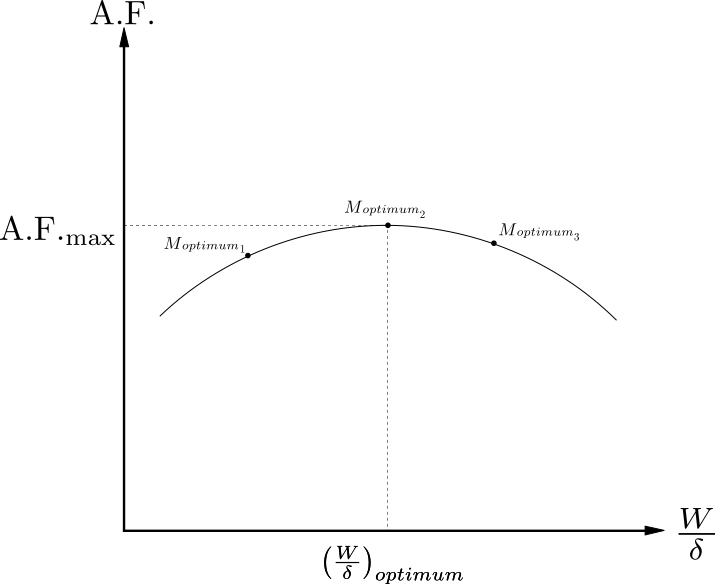
\includegraphics[keepaspectratio, width=0.60\textwidth]{AutonomyFactor}
\caption{Autonomy factor trend as function of the generalized weight}
\label{fig:Figure5}
\end{figure}

\noindent
As can be seen from figure~\ref{fig:Figure5} the autonomy factor has a maximum at a specific generalized weight which is the one that the pilot should maintain during the cruise phase. 

If the altitude is fixed, and so $\delta$ is constant, the chart in figure~\ref{fig:Figure5} can be seen as function of Mach number for a given aircraft weight; at this point, knowing that the autonomy factor leads to the specific range if divided by the aircraft weight, it's possible to define the specific range trend as funcion of the Mach number parameterized in aircraft weight. 

\begin{figure}[b]
\centering
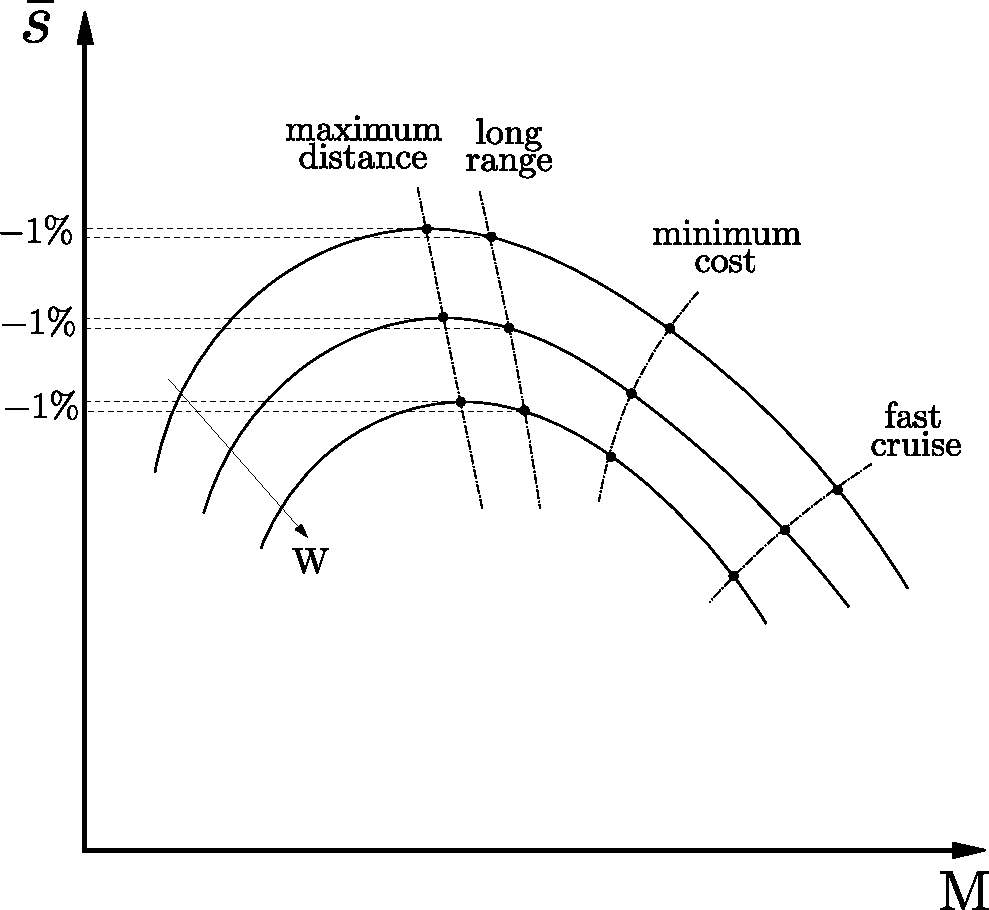
\includegraphics[keepaspectratio, width=0.50\textwidth]{CruiseGrid}
\caption{Specific range as function of the Mach number parameterized in aricraft weight}
\label{fig:Figure6}
\end{figure}

\bigskip
\noindent
The chart, so obtained, in figure~\ref{fig:Figure6} is the one upon which the cruise grid is defined; on the latter, in fact, four lines are drawn each of which is related to a precise mission objecive.

It's important to highlight that, on long distances, the maximum distance line is not often followed during the cruise because it is tied to a low speed which adversely affects the total flight time increasing the D.O.C.; in order to avoid this condition, pilots prefer to follow the long range line which has only 1\% of penalty on the specific range but, at the same time, allows to fly at significantly higher speed with benefits on flight time and, as a result, on the~D.O.C.

%------------------------- JAVA CLASS ARCHITECTURE ---------------------------

\section{Java class architecture}
After having introduced the theory behind the cruise grid chart, a presentation of the related Java class inside JPAD is shown. Using the same philosophy of the previous chapter, a dedicated class, named \lstinline[language=Java]!SpecificRangeCalc!, has been implemented inside which a series of static methods provide the needed calculation tools. Generaly speaking, the giudeline followed in creating this class is to assign an array of Mach numbers, starting from the one realitve to the minimum cruising speed and ending with the maximum cruising speed at that altitude and weight, and then evaluate the SFC, from engine database, for each Mach number; from here the A.F. is built after the evaluation of the aerodynamic efficinecy for each value of the same Mach array. Finally the specific range is calculated, in $\frac{\si{nmi}}{\si{lbs}}$, dividing the A.F. by the aircraft max take off mass.

\bigskip
\noindent
The first static method presented is \lstinline[language=Java]!calculateEfficiencyVsMach!. It allows to evaluate the aerodynamic efficiency value for each  Mach number of a given array through the evaluation of the C\textsubscript{L} and the relative C\textsubscript{D} from the aircraft total drag polar; in particular the two aerodynamic coefficients are calculated by calling other two static methods which come from two classes of the aerodynamic calculator package of \lstinline[language=Java]!JPADCore! named, respectively, \lstinline[language=Java]!LiftCalc! and \lstinline[language=Java]!DragCalc!.

The static \lstinline[language=Java]!LiftCalc! method, named \lstinline[language=Java]!calculateLiftCoeff!, performs the C\textsubscript{L} calculation using the following formula, valid in cruise phase.

\begin{equation}
C_L=\frac{2W}{\rho S V^2}
\label{eqn:Lift.Equation}
\end{equation}

\noindent
where $V$, is the TAS speed derived from the actual Mach number of the array at that the given altitude.

\begin{table}[b]
\begin{tabular}{p{7cm}p{7.5cm}}
\toprule
\lstinline[language=Java]!maxTakeOffMass! & Maximum take-off mass \\[0.1	cm]
\lstinline[language=Java]!sweepHalfChordEquivalent! & Equivalent wing sweep angle at half chord \\[0.1cm]
\lstinline[language=Java]!surface! & Wing surface \\[0.1cm]
\lstinline[language=Java]!cd0!	& Wing c\textsubscript{D0} \\[0.1cm]
\lstinline[language=Java]!oswald!	& Wing oswald factor \\[0.1cm]
\lstinline[language=Java]!mach!	& An array of Mach numbers \\[0.1cm]
\lstinline[language=Java]!ar!	& Wing aspect ratio \\[0.1cm]
\lstinline[language=Java]!tcMax! & Mean maximum thickness of the wing \\[0.1cm]
\lstinline[language=Java]!altitude! & Cruise altitude \\[0.1cm]
\lstinline[language=Java]!airfoilType! & The wing airfoil type from the related \lstinline[language=Java]!AirfoilType! enumeration \\
\bottomrule
\end{tabular}
\caption{ \lstinline[language=Java]!calculateEfficiencyVsMach! input data}
\label{table:Table1}
\end{table}

On the other hand, the static \lstinline[language=Java]!DragCalc! method, named \lstinline[language=Java]!calculateCDTotal!, performs the C\textsubscript{D} calculation using the total drag polar expression.

\begin{equation}
C_D=C_{D0}+\frac{C_L^2}{\pi \ensuremath{\AR} e}+C_{Dwave}
\label{eqn:Drag.Total}
\end{equation}

\bigskip
\noindent
~where the $C_{Dwave}$ is calculated as presented in~\cite{hilton1951high}.

\bigskip
\noindent
The second static method implemented is \lstinline[language=Java]!calculateSfcVsMach!, which accepts as input data reported in table~\ref{table:Table2} allows to evaluate the SFC of a turboprop aircraft, or the SFCJ of a turbofan aircraft, for each Mach number of the given array by reading data from the related engine database.

\begin{table}[t]
\begin{tabular}{p{7cm}p{7.5cm}}
\toprule
\lstinline[language=Java]!mach!	& An array of Mach numbers \\[0.1cm]
\lstinline[language=Java]!altitude! & Cruise altitude \\[0.1cm]
\lstinline[language=Java]!bpr! & Engine By-Pass ratio \\[0.1cm]
\lstinline[language=Java]!engineType! & The engine type from the related \lstinline[language=Java]!EngineType! enumeration \\
\bottomrule
\end{tabular}
\caption{ \lstinline[language=Java]!calculateSfcVsMach! input data}
\label{table:Table2}
\end{table}

\bigskip
\noindent
Finally, the two previous method leads to the last one named \lstinline[language=Java]!calculateSpecificRangeVsMach! which allows to calculate the A.F. and, from it, the specific range by implementing the (\ref{eqn:AutonomyFactorProp}) or the (\ref{eqn:AutonomyFactorJet}) depending on the given engine type. 

To do this, it's necessary to give as input the Mach numbers array, the aerodynamic efficiency array calculated with~\lstinline[language=Java]!calculateEfficiencyVsMach! and the SFC array calculated with~\lstinline[language=Java]!calculateSfcVsMach! as shown in table~\ref{table:Table3}.

\begin{table}[!b]
\begin{tabular}{p{7cm}p{7.5cm}}
\toprule
\lstinline[language=Java]!maxTakeOffMass! & Maximum take-off mass \\[0.1	cm]
\lstinline[language=Java]!mach!	& An array of Mach numbers \\[0.1cm]
\lstinline[language=Java]!efficiency!	& An array of aerodynamic efficiency values \\[0.1cm]
\lstinline[language=Java]!sfc!	& An array of SFC values \\[0.1cm]
\lstinline[language=Java]!bpr! & Engine By-Pass ratio \\[0.1cm]
\lstinline[language=Java]!altitude! & Cruise altitude \\[0.1cm]
\lstinline[language=Java]!eta!	& Propeller efficiency (set to zero in case of turbofan) \\[0.1cm]
\lstinline[language=Java]!engineType! & The engine type from the related \lstinline[language=Java]!EngineType! enumeration \\
\bottomrule
\end{tabular}
\caption{ \lstinline[language=Java]!calculateSpecificRangeVsMach! input data}
\label{table:Table3}
\end{table}

\bigskip
\noindent
The class is completed by other four static methods demanded of plotting the results; in particular, using the same approach shown in the previous chapter, a .png and a .tikz output images are created for each of the SFC, the aerodynamic efficiency and the specific range.

It's important to highlight that the first of these plotting methods, which is named \lstinline[language=Java]!createSpecificRangeChart! and is demanded of plotting the cruise grid chart, has implemented, inside it, the evaluation of the maximum range condition as well as the long range one; this by calculating all maximum points and, from them, all points at -1\% of penalty obtained through the evaluation of the bigger of the two intersction points that the line at -1\% of penalty defines on each specific range curve.

\noindent
The fourth method is, insetad, used for plotting the intersection between the required and available thrust, giving as input a speed array, the altitude and two~\lstinline[language=Java]!List! of custom~\lstinline[language=Java]!Map! named~\lstinline[language=Java]!DragMap! and~\lstinline[language=Java]!ThustMap!; these are two classes used to store all data related to drag and thrust curves like the aircraft weight, the current altitude, the speed array on which the drag or thrust are evaluated and, finally, the drag or thrust array itself.  

\bigskip
\noindent
In conclusion a flowchart of the described class is shown in figure~\ref{fig:Figure7} in order to simplify its understanding.

\begin{figure}[t]
\centering
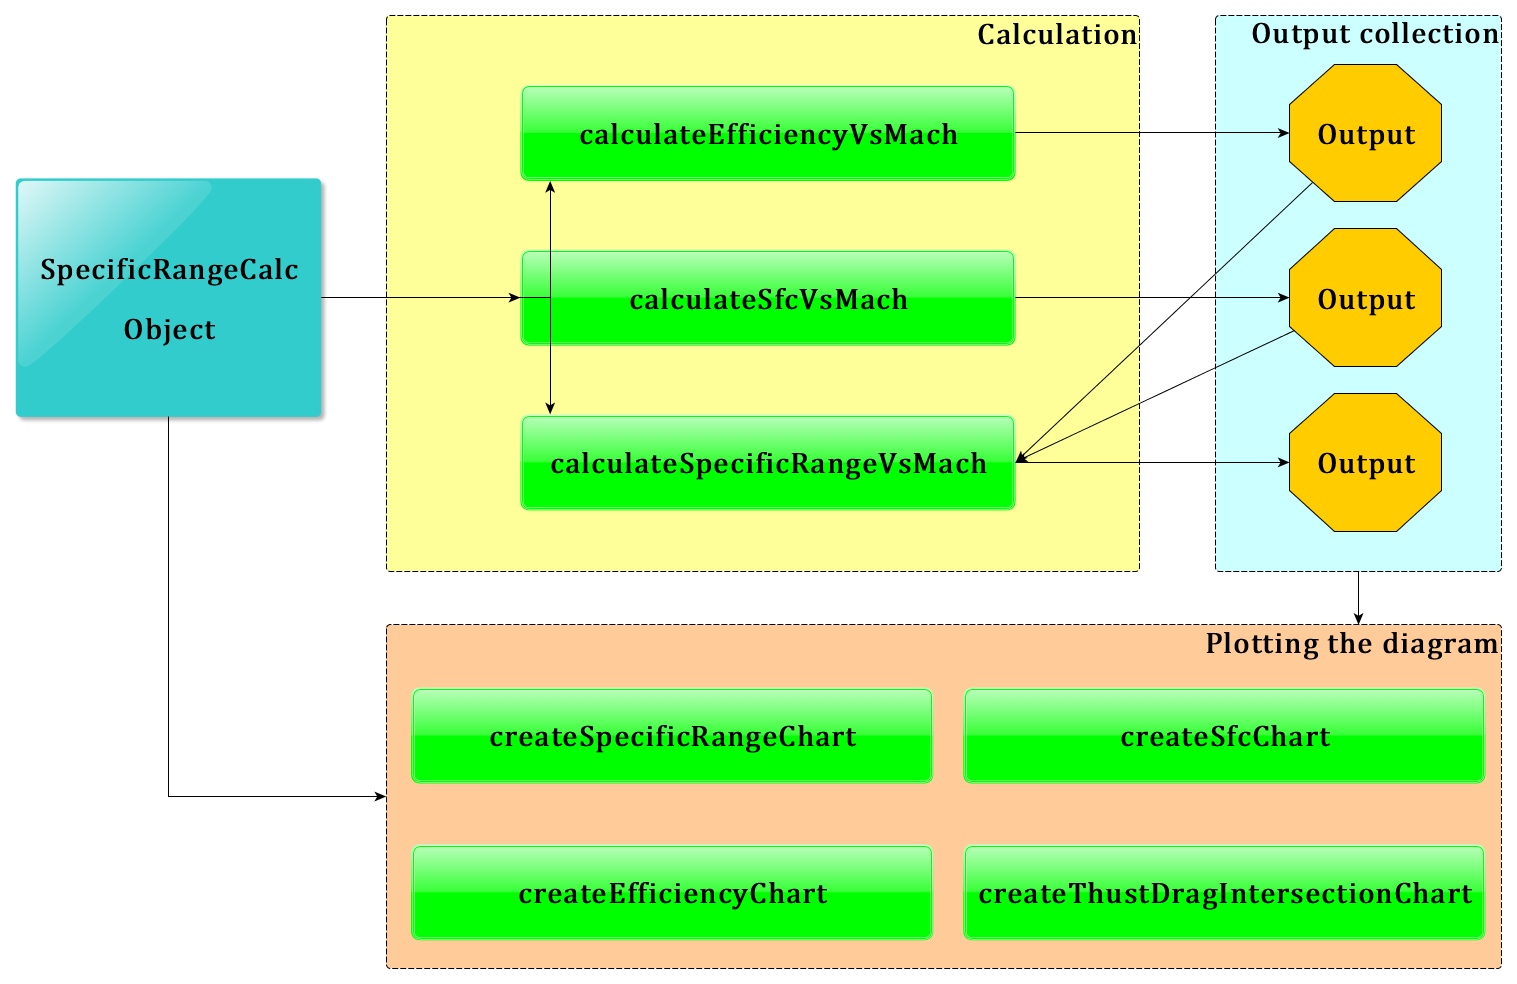
\includegraphics[keepaspectratio, width=0.90\textwidth]{SpecificRange_Flowchart}
\caption{\lstinline[language=Java]!SpecificRangeCalc! class flowchart}
\label{fig:Figure7}
\end{figure}

%----------------------- CASE STUDY : ATR72 AND B747 -------------------------
\section{Case study: ATR-72 and B747-100B}

In order to validate all the teoretical concepts explained in the previous paragraphs, as well as to give to the reader a useful example of how to handle this class usage, the following pages shows two application of the class methods made upon the two default aircraft described in paragraph~\ref{par:DefultAircraft}.

\bigskip
\noindent
Once all preliminary steps have been completed, as explained in paragraph~\ref{par:DefultAircraft}, it's possible to start the test of this class. 

First of all, since the cruise grid chart is parameterized in aircraft weight, an array of aircraft masses has to be created; in particular, in this test, a variation of mass of -10\% has been implemented, starting from the aircraft maximum take-off mass until it reaches the 60\% of the latter. 

The second step is to define the independent variable, which is the Mach number, and in particular it's necessary to identify the upper and lower limitations of its array; this can be done by evaluating the required thrust, which is equal to the drag during cruise, and comparing it with the available thrust supplied by the power plant.

\noindent
By the intersections of the latter, the two required speeds can be derived; otherwise, if the minimum speed intersection can't be found, the cruising stalling speed, at that weight and altitude condition and for a specified c\textsubscript{Lmax}, replaces the missing intersection abscissa.

\begin{figure}[t]
\begin{lstlisting}[caption={Mass variation in Specific Range test - B747-100B}, captionpos=b, tabsize=2]
		double[] maxTakeOffMassArray = new double[5];
		for (int i=0; i<5; i++)
		
			maxTakeOffMassArray[i] =
							aircraft.get_weights().get_MTOM().plus(aircraft.get_weights().get_MLM()).divide(2).getEstimatedValue()
							*(1-0.1*(4-i));

		double[] weight = new double[maxTakeOffMassArray.length];
		for(int i=0; i<weight.length; i++)
			weight[i] = maxTakeOffMassArray[i]*AtmosphereCalc.g0.getEstimatedValue();
\end{lstlisting}
\end{figure}

In terms of code, the last step can be carried out using the static method~\lstinline[language=Java]!calculateDragThrustIntersection! of the~\lstinline[language=Java]!JPADCore! class named~\lstinline[language=Java]!PerformanceCalcUtils!; the latter requires as input the following data:

\begin{itemize}
\item An array of altitudes
\item An array of speeds
\item An array of weights
\item An array of throttle settings
\item An array of flight conditions chosen from a dedicated enumeration named~\lstinline[language=Java]!EngineOperatingConditionEnum!
\item The engine by-pass ratio, set to zero in case of propeller aircraft
\item The wing surface
\item Wing C\textsubscript{Lmax} in clean configuration
\item A~\lstinline[language=Java]!List! of custom data map named~\lstinline[language=Java]!DragMap!
\item A~\lstinline[language=Java]!List! of custom data map named~\lstinline[language=Java]!ThrustMap!
\end{itemize}

%---------------------------ADD DRAG AND THUST MAP DESCRIPTION THEN CONTINUE TO EXPLAIN THE TEST----------------------------------------------------

